% Vākya-Vallarī paper — compile: pdflatex -> bibtex -> pdflatex -> pdflatex
\documentclass[11pt]{article}

\usepackage[margin=1.05in]{geometry}
\usepackage[utf8]{inputenc}
\usepackage[T1]{fontenc}
\usepackage{lmodern}
\usepackage{microtype}
\usepackage{natbib}
\usepackage{booktabs}
\usepackage{graphicx}
\usepackage{tikz}
\usepackage{pgfplots}
\pgfplotsset{compat=1.18}
\usetikzlibrary{shapes.geometric, arrows.meta, positioning, fit, calc, backgrounds}
\usepackage{listings}
\usepackage{amsmath, amssymb, amsthm}
\usepackage{xcolor}
\usepackage[colorlinks=true, linkcolor=blue!50!black, citecolor=blue!50!black, urlcolor=blue!50!black]{hyperref}

% IAST diacritics under pdflatex
\DeclareUnicodeCharacter{0101}{\=a}   % ā
\DeclareUnicodeCharacter{012B}{\={\i}}% ī
\DeclareUnicodeCharacter{016B}{\=u}   % ū
\DeclareUnicodeCharacter{1E5B}{\d{r}} % ṛ
\DeclareUnicodeCharacter{1E63}{\d{s}} % ṣ
\DeclareUnicodeCharacter{1E6D}{\d{t}} % ṭ
\DeclareUnicodeCharacter{1E0D}{\d{d}} % ḍ
\DeclareUnicodeCharacter{1E47}{\d{n}} % ṇ
\DeclareUnicodeCharacter{1E25}{\d{h}} % ḥ
\DeclareUnicodeCharacter{1E43}{\d{m}} % ṃ
\DeclareUnicodeCharacter{015B}{\'s}   % ś
\DeclareUnicodeCharacter{00F1}{\~n}   % ñ
\DeclareUnicodeCharacter{1E45}{\.n}   % ṅ

\definecolor{leanbg}{RGB}{246,241,231}
\lstdefinelanguage{lean}{
  keywords={theorem, def, structure, inductive, namespace, end, import, open, by, decide, deriving, where, example},
  sensitive=true, comment=[l]{--},
}
\lstset{basicstyle=\small\ttfamily, keywordstyle=\bfseries, commentstyle=\itshape\color{gray},
        frame=single, backgroundcolor=\color{leanbg!50}, breaklines=true, captionpos=b,
        literate={ā}{{\=a}}1 {ī}{{\={\i}}}1 {ṛ}{{\d{r}}}1 {ṣ}{{\d{s}}}1 {ṭ}{{\d{t}}}1
                 {ḍ}{{\d{d}}}1 {ṇ}{{\d{n}}}1 {ḥ}{{\d{h}}}1 {ṃ}{{\d{m}}}1 {ś}{{\'s}}1
                 {≠}{{$\neq$}}1 {¬}{{$\neg$}}1 {⟨}{{$\langle$}}1 {⟩}{{$\rangle$}}1 {→}{{$\to$}}1
                 {∧}{{$\wedge$}}1 {∨}{{$\vee$}}1 {│}{{|}}1}

\newtheorem{definition}{Definition}

\title{Machine-Checked Translation Adequacy for Bhart\d{r}hari's
  \emph{V\={a}kyapad\={\i}ya}:\\ Commentary-Driven Verification of a Sanskrit
  Philosophical Text in Lean~4}

\author{Sharath Sathish\\
  \small with an agentic formalization loop built on Claude (Anthropic)\\
  \small \url{https://github.com/SharathSPhD/vakya-vallari}}

\date{July 2026}

\begin{document}
\maketitle

\begin{abstract}
Translations of dense philosophical Sanskrit are notoriously under-determined:
a single k\={a}rik\={a} admits multiple grammatically valid renderings whose
philosophical commitments differ radically, and the commentarial tradition ---
not surface grammar --- is what fixes the intended reading. We introduce
\emph{commentary-driven translation validation} (C-TV), to our knowledge the
first application of an interactive theorem prover to translation adequacy in
linguistics, and apply it to the complete Brahmak\={a}\d{n}\d{d}a (Book~I, 144
verse units) of Bhart\d{r}hari's \emph{V\={a}kyapad\={\i}ya}. From an original
English translation and analytical commentary of all 1,796 verses we derive,
per verse, a \emph{semantic contract}: sorted entities, identity, relation and
predication claims, and explicit denials, every axiom citing the commentary
verbatim --- a mechanical anti-fabrication gate. A generator compiles contracts
into Lean~4, where a decidable adequacy predicate proves that the accepted
translation satisfies the contract (144 adequacy theorems) and that 350
plausible mistranslations provably fail --- 153 contradicted by commentary
denials, 197 unlicensed by the axioms --- for 549 machine-checked theorems with
zero \texttt{sorry}. The corpus was formalized by an agentic swarm gated by the
validator and the Lean kernel; the gates caught real errors at every scale,
from fabricated citations in degraded agent output to cross-contract
ontological drift, adjudicated into a registry of 41 polysemous terms with 91
textually justified senses --- including the ak\d{s}ara pun that
Bhart\d{r}hari's own commentators call the argument of the opening verse in
miniature. A GPU embedding audit of all 1,796 translation--commentary pairs
provides a corpus-scale review queue that correlates with independently flagged
contested readings. We state precisely what is and is not verified: Lean checks
the internal coherence of the formalization against the commentary-derived
contract; the contract--commentary link remains human-auditable by
construction, through verbatim citations. All artifacts --- corpus, contracts,
kernel, proofs, edition --- are public and reproducible.
\end{abstract}

\section{Introduction}
\label{sec:intro}

The \emph{V\={a}kyapad\={\i}ya} (``Treatise on Sentence and Word,''
c.~5th century CE) is the foundational text of Indian philosophy of language.
Its opening verse already illustrates the problem this paper addresses:

\begin{quote}
\emph{an\={a}dinidhana\d{m} brahma \'sabdatattva\d{m} yadak\d{s}aram\,/\\
vivartate'rthabh\={a}vena prakriy\={a} jagato yata\d{h}\,//} (VP 1.1)
\end{quote}

A translator must decide whether \emph{\'sabdatattva} (``word-essence'') is a
\emph{property of language} or \emph{the Absolute itself}; whether
\emph{vivartate} means the world is a \emph{transformation} of Brahman
(pari\d{n}\={a}ma) or its \emph{appearance without transformation} (vivarta);
and whether \emph{ak\d{s}ara} means ``imperishable,'' ``phoneme,'' or ---
as the grammarian tradition insists --- deliberately both. Each choice yields a
grammatical English sentence; the choices differ philosophically as much as
materialism differs from idealism. What disambiguates them is not syntax but
the commentarial tradition: the vast apparatus of v\d{r}tti and
\d{t}\={\i}k\={a} that fixes, verse by verse, which reading the text licenses
\citep{iyer1965vakyapadiya, houben2016vakyapadiya}.

Translation of such texts has therefore been an art form in which the
constraints, though real, live only in the philologist's head. This paper makes
them mechanical. Our claim is not that a theorem prover can read Sanskrit; it
is that once a scholar's interpretive commitments are stated as data, a
proof assistant can \emph{hold the translation to them} --- exhaustively,
incrementally, and publicly.

\paragraph{Contributions.}
\begin{enumerate}
  \item \textbf{Commentary-driven translation validation (C-TV).} We adapt
    translation validation from compiler verification
    \citep{pnueli1998translation, leroy2009compcert, tristan2008validators} to
    natural language: the commentary is compiled into per-verse \emph{semantic
    contracts} (\S\ref{sec:contracts}), and a translation's reading is verified
    against the contract, not against the bare source string. To our knowledge
    this is the first application of an interactive theorem prover to
    translation adequacy in linguistics, and the first mechanized treatment of
    any Sanskrit philosophical text.\footnote{Prior mechanizations of Indian
    logic formalize the logical \emph{systems} (\S\ref{sec:related}); none, to
    our knowledge, verifies \emph{translations of texts}.}
  \item \textbf{A verified Brahmak\={a}\d{n}\d{d}a.} All 144 verse units of
    Book~I carry compiled adequacy theorems, and 350 plausible mistranslations
    are \emph{compiled counterexamples} --- refuted by theorem, not by footnote
    (\S\ref{sec:kernel}). The full corpus of 1,796 verses with original
    translation and commentary is released as a checksummed, schema-validated
    digital edition.
  \item \textbf{An anti-fabrication architecture for agentic formalization.}
    The contracts were authored by an LLM-agent swarm, and every layer is
    gated: axioms must cite the commentary \emph{verbatim}; rejected readings
    must \emph{provably} fail; entity sorts must be globally consistent or
    adjudicated as polysemy in a justified registry (\S\ref{sec:loop},
    \S\ref{sec:ontology}). We report what the gates caught --- including
    fabricated citations in quota-degraded agent output --- as evidence that
    the architecture, not agent goodwill, carries the epistemic load.
  \item \textbf{A corpus-scale semantic audit.} A GPU embedding pass over all
    1,796 translation--commentary pairs yields a drift-ranked review queue
    that correlates with the edition's independently flagged \emph{contested}
    readings (\S\ref{sec:audit}).
\end{enumerate}

\section{Background and Related Work}
\label{sec:related}

\paragraph{Bhart\d{r}hari and the spho\d{t}a doctrine.}
The \emph{V\={a}kyapad\={\i}ya} comprises three books
(Brahmak\={a}\d{n}\d{d}a, V\={a}kyak\={a}\d{n}\d{d}a, Padak\={a}\d{n}\d{d}a).
Book~I develops \'sabd\={a}dvaita --- the thesis that the Absolute is of the
nature of the word --- and the spho\d{t}a doctrine: the meaning-bearing word is
an undivided whole, merely \emph{manifested} by the temporal sequence of
sounds \citep{coward1980sphota, biardeau1964theorie, staal1969sanskrit}.
Both doctrines generate exactly the translation hazards our system checks:
sort errors (demoting the Absolute to a property), relation errors
(rendering manifestation as transformation), and homonym errors (collapsing
the technical senses of ak\d{s}ara, spho\d{t}a, dhvani).

\paragraph{Computational Sanskrit.}
P\={a}\d{n}inian grammar has long been recognized as a formal generative
system \citep{kiparsky2009panini, cardona1976panini, scharf2009panini}, and a
mature computational ecosystem exists for segmentation, morphology and
generation \citep{goyal2016samsaadhanii, hellwig2020sanskrit, vidyut}, with
TEI-encoded editions in SARIT \citep{sarit}. This work is orthogonal and
complementary: we verify \emph{semantics against commentary}, not surface
analysis.

\paragraph{Formalizing Indian logic.}
Navya-Ny\={a}ya has been studied logically since
\citet{ingalls1951materials} and \citet{matilal1968navya}; recently
\citet{panday2026cubical} encoded its core constructs (relational nesting,
delimitors, typed absence) in cubical type theory, \citet{sathish2026pramana}
trained LLMs on its six-phase epistemic method, and \citet{diehl2024fourfold}
mechanized the Buddhist catu\d{s}ko\d{t}i in Lean. These formalize the
\emph{logics}; none verifies translations of a text. Our kernel borrows
Navya-Ny\={a}ya's structural insights (\S\ref{sec:kernel}) in plain Lean~4
\citep{demoura2021lean4}, without cubical machinery.

\paragraph{Translation validation and autoformalization.}
Translation validation checks each compiler run \emph{a posteriori} instead of
verifying the compiler \citep{pnueli1998translation, tristan2008validators}.
We transplant the pattern: the human translator is the untrusted optimizer;
the contract is the semantic reference; Lean is the validator. On the
authoring side, LLM autoformalization \citep{wu2022autoformalization,
pathak2024gflean} supplies the untrusted draft whose output the kernel gates
--- our loop is an instance of the generate-and-check paradigm with an
unusually strict checker.

\section{The Corpus}
\label{sec:corpus}

The edition is built from two sources: (i) the Devanagari m\={u}la
k\={a}rik\={a}s scraped from a public edition (wisdomlib.org), and (ii) an
original English translation and analytical commentary of every verse, written
from the Sanskrit for this project. Alignment is checked, never assumed: the
1,796 commentary units (144 / 426 / 1,226 per book) are the canonical keys;
every unit must match a m\={u}la entry by exact label or be quarantined with a
reason. The build is test-driven (12 corpus gates), and the tests forced three
philologically real discoveries: the \emph{contested} field is a prose note
explaining each disputed reading (286 verses), not a boolean; verse markers
legitimately embed Latin half-verse letters; and the source edition assigns
the label 2.127cd to two different pages --- a defect the commentary itself
documents, which the loader merges and flags rather than silently overwriting.
The resulting JSONL corpus carries per-record provenance and a manifest with a
SHA-256 checksum.

\begin{table}[t]
\centering
\caption{The V\={a}kya-Vallar\={\i} corpus and the verified subset
(Brahmak\={a}\d{n}\d{d}a complete).}
\label{tab:corpus}
\begin{tabular}{lrrrr}
\toprule
 & \textbf{Book I} & \textbf{Book II} & \textbf{Book III} & \textbf{Total} \\
\midrule
Verse units (canonical)        & 144 & 426 & 1,226 & 1,796 \\
Contested readings (prose notes) & 56 & 167 & 63 & 286 \\
Semantic contracts             & 144 & --- & --- & 144 \\
Adequacy theorems (Lean)       & 144 & --- & --- & 144 \\
Refutation theorems (Lean)     & 350 & --- & --- & 350 \\
\bottomrule
\end{tabular}
\end{table}

\section{Semantic Contracts}
\label{sec:contracts}

\begin{definition}[Semantic contract]
A contract for verse $v$ is a JSON document with (i) \emph{entities}: named
terms with ontological sorts drawn from $\{$absolute, power, manifestation,
linguisticItem, property, cognition$\}$; (ii) \emph{axioms} and
\emph{denials}: identity, relation and predication claims over those entities,
each carrying a citation that must occur \emph{verbatim} in the verse's
commentary; (iii) an \emph{accepted reading}: the claims the translation
asserts, each citing the translation verbatim; and (iv) \emph{rejected
readings}: plausible mistranslations rendered as claim sets, each annotated
with the failure mode it must exhibit --- \texttt{contradicted} (asserts a
denial) or \texttt{unlicensed} (asserts what no axiom entails).
\end{definition}

The verbatim-citation rule is the anti-fabrication gate: an axiom that cannot
point to the commentary text that licenses it is rejected mechanically, before
any proof is attempted. Across the 144 contracts there are 772 entity
declarations, 610 axioms, 178 denials, 449 accepted-reading claims and 350
rejected readings. The validator further checks sort membership, ASCII
identifier hygiene (a Lean requirement discovered the hard way,
\S\ref{sec:loop}), entailment of the accepted reading, and provable failure of
every rejected reading --- the last via the same decision procedure the Lean
kernel uses, so that Python-side acceptance predicts Lean-side theoremhood.

\section{The Lean Kernel}
\label{sec:kernel}

The kernel (\texttt{VakyaVallari}, Lean~4.32, no external dependencies) is
deliberately small. Entities are sort-tagged terms; claims are inductive data;
a contract is axioms plus denials; and adequacy is \emph{decidable}, so every
verse-level theorem closes by \texttt{decide} --- the proof term is the
computation.

\begin{lstlisting}[language=lean, caption={Core of the adequacy kernel (abridged).}]
inductive Sorta | absolute | power | manifestation
               | linguisticItem | property | cognition
structure Entity where  name : String;  sort : Sorta
-- paramparā: a relation can itself be a relatum, to any depth
inductive Node | ent : Entity → Node
              | rel : String → Node → Node → Node
structure Abhava where  pratiyogin : Node;  adhikarana : Node
structure Contract where  axioms : List Claim;  denials : List Claim
def Adequate (c : Contract) (r : Reading) : Prop :=
  r.claims.all (entails c.axioms) ∧ ¬ r.claims.any (denied c.denials)
\end{lstlisting}

Three Navya-Ny\={a}ya-inspired choices matter. \emph{Sorted identity}: claims
of identity are stateable across sorts but decidably false when sorts differ,
so a mistranslation that demotes the Absolute to a property fails by
\emph{sort error} --- the C-TV failure mode as a computation. \emph{Nested
relations}: \texttt{Node} makes relations first-class relata
(parampar\={a}-sambandha), so ``Time is the instrumental cause \emph{of the
manifestation-relation}'' is representable without ad hoc reification.
\emph{Typed absence}: \texttt{Abhava} carries its counterpositive and locus as
data, and the kernel proves Raghun\={a}tha's involution (the absence of an
absence computes to the presence) as a definitional fact.

Each contract compiles to a Lean module in which the accepted reading's
adequacy is a theorem and every rejected reading's failure is a theorem.
Verse 1.1's module ends, in full:

\begin{lstlisting}[language=lean, caption={Generated theorems for VP 1.1 (excerpt).}]
theorem accepted_adequate : contract.Adequate accepted := by decide
-- "The imperishable linguistic structure underlying words..."
theorem naive_linguistic_structure_inadequate :
    ¬ contract.Adequate naive_linguistic_structure := by decide
theorem naive_linguistic_structure_sort_error :
    sabdatattva_naive ≠ sabdatattva := by decide
-- "Brahman transforms itself into the world of objects."
theorem parinama_transformation_inadequate :
    ¬ contract.Adequate parinama_transformation := by decide
\end{lstlisting}

The build gate is binary and global: \texttt{lake build} must succeed with
zero \texttt{sorry} across all 144 modules --- 549 theorems at present. A
counterexample that stops compiling is a regression, caught in CI.

\paragraph{Honesty boundary.}
Lean verifies the \emph{internal coherence of the formalization}: that the
accepted reading satisfies the contract and rivals do not. Whether the
contract is faithful to Bhart\d{r}hari is not a theorem and cannot be one; it
is a human-auditable question, and the system is built so that the audit is
cheap --- every axiom links to the exact commentary sentence it derives from.
We regard this boundary not as a limitation to apologize for but as the
correct division of labor between prover and philologist.

\begin{figure}[t]
\centering
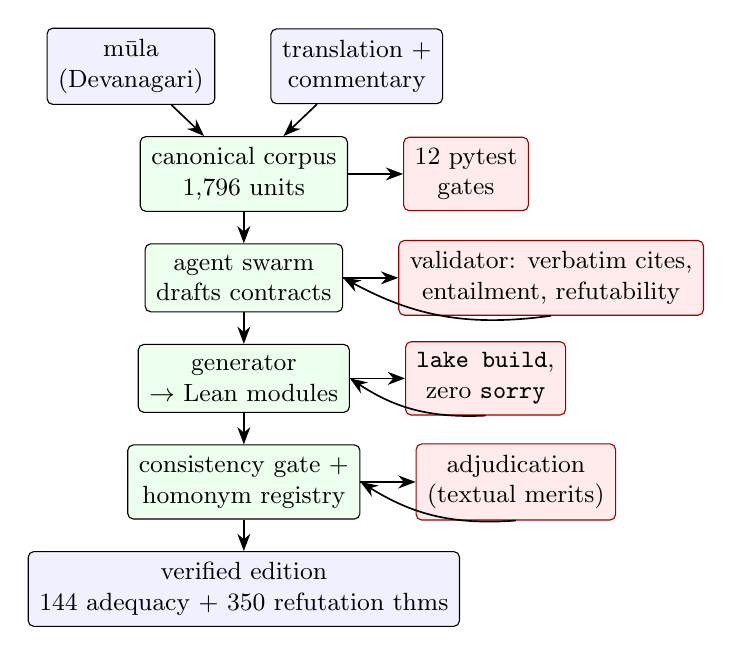
\begin{tikzpicture}[
  node distance=4mm and 7mm,
  box/.style={draw, rounded corners=2pt, align=center, font=\small,
              inner sep=4pt, minimum height=8.5mm},
  gate/.style={box, fill=red!8, draw=red!60!black},
  data/.style={box, fill=blue!6},
  proc/.style={box, fill=green!7},
  arr/.style={-{Stealth[length=2.2mm]}, semithick}]
\node[data] (mula) {m\={u}la\\ (Devanagari)};
\node[data, right=of mula] (comm) {translation +\\ commentary};
\node[proc, below=of $(mula.south)!0.5!(comm.south)$] (corpus)
  {canonical corpus\\ 1,796 units};
\node[gate, right=of corpus] (g1) {12 pytest\\ gates};
\node[proc, below=of corpus] (swarm) {agent swarm\\ drafts contracts};
\node[gate, right=of swarm] (g2) {validator: verbatim cites,\\ entailment, refutability};
\node[proc, below=of swarm] (leangen) {generator\\ $\to$ Lean modules};
\node[gate, right=of leangen] (g3) {\texttt{lake build},\\ zero \texttt{sorry}};
\node[proc, below=of leangen] (adj) {consistency gate +\\ homonym registry};
\node[gate, right=of adj] (g4) {adjudication\\ (textual merits)};
\node[data, below=of adj] (out) {verified edition\\ 144 adequacy + 350 refutation thms};
\draw[arr] (mula) -- (corpus);
\draw[arr] (comm) -- (corpus);
\draw[arr] (corpus) -- (g1);
\draw[arr] (corpus) -- (swarm);
\draw[arr] (swarm) -- (g2);
\draw[arr] (g2.south) to[bend left=18] (swarm.east);
\draw[arr] (swarm) -- (leangen);
\draw[arr] (leangen) -- (g3);
\draw[arr] (g3.south) to[bend left=18] (leangen.east);
\draw[arr] (leangen) -- (adj);
\draw[arr] (adj) -- (g4);
\draw[arr] (g4.south) to[bend left=18] (adj.east);
\draw[arr] (adj) -- (out);
\end{tikzpicture}
\caption{The C-TV pipeline. Every layer has a mechanical gate (red); failures
feed back as repair work, and the append-only research ledger records each
draft, rejection, repair and acceptance.}
\label{fig:pipeline}
\end{figure}

\section{The Agentic Formalization Loop}
\label{sec:loop}

Contracts were authored by an LLM-agent swarm --- one agent per verse, each
given the verse record, the schema, an exemplar, and the validator as its exit
gate --- orchestrated in rounds of 9--30 agents with an adjudication pass
between rounds and an append-only ledger (96 events) recording every draft,
rejection, repair and acceptance. The division of labor is the point: agents
propose; gates dispose. Four episodes illustrate what the gates caught.

\begin{table}[t]
\centering
\caption{Errors caught mechanically during formalization. ``Lazy
counterexample'' = a rejected reading whose claims were secretly entailed;
``fabricated citation'' = an axiom cite absent from the commentary.}
\label{tab:catches}
\begin{tabular}{lrl}
\toprule
\textbf{Failure class} & \textbf{Count} & \textbf{Caught by} \\
\midrule
Lazy counterexamples             & 3 & Lean kernel, then hardened validator \\
Fabricated / paraphrased citations & 5 & verbatim-cite gate \\
Non-ASCII Lean identifiers       & 2 contracts & Lean parser, then validator \\
Cross-contract sort drift        & 89 conflicts & consistency gate \\
Diacritic name splits (spho\d{t}a/sphota) & 2 episodes & consistency gate \\
\bottomrule
\end{tabular}
\end{table}

\emph{(i) Lazy counterexamples.} Early agents produced rejected readings that
merely restated axioms --- theorems of inadequacy would have been false. The
Lean build failed; the validator was hardened to require provable failure; three
contracts were repaired.

\emph{(ii) Fabricated citations under degradation.} When an API session limit
killed 20 of 30 agents mid-round, 9 left unreviewed draft contracts. Five of
the nine failed the verbatim-citation gate --- paraphrased or invented cites.
This is the anti-fabrication architecture functioning as designed: degraded
generation was caught by the gate, quarantined, and re-authored cleanly.

\emph{(iii) Identifier hygiene.} Lean's parser rejected IAST diacritics in
entity identifiers that Python's \texttt{isidentifier()} accepts; the
validator now enforces ASCII identifiers, and the incident is a small argument
for keeping the end-to-end kernel gate even when a faster mirror exists.

\emph{(iv) Sort drift.} Independent agents assigned different sorts to the
same term. Across five adjudication rounds the consistency gate surfaced 89
conflicts; adjudication (below) resolved each as either a correction or
genuine polysemy.

\section{Ontological Consistency and the Homonym Registry}
\label{sec:ontology}

The corpus-level gate requires that a named entity carry one sort everywhere
--- unless the exact partition of (verse, sort) uses is registered as
polysemy, with a gloss and a one-sentence textual justification per sense. The
registry now holds 41 terms with 91 senses, and it is where the method earns
its keep philologically: the gate cannot tell drift from doctrine, so every
split is a documented editorial ruling.

Three registered splits are load-bearing. \emph{ak\d{s}ara}: the imperishable
Absolute in 1.9 versus phoneme in 1.18--22 --- the pun the commentary calls
``the argument in miniature'' of verse 1.1, which a same-sort rule would have
flattened. \emph{\'sabda}: linguisticItem canonically, but the Absolute in the
fire-in-wood verse (1.46), where the inner word is \'sabdatattva itself.
\emph{spho\d{t}a}: linguisticItem in Bhart\d{r}hari's own doctrine, but
verses 1.102--1.106 \emph{report a rival phonetician terminology} in which
spho\d{t}a names the first-produced acoustic sound --- a distinct sense
(manifestation) covering exactly the doxographic span, keeping the report from
contaminating the doctrine.

\section{Corpus-Scale Semantic Audit}
\label{sec:audit}

Formal verification covers Book~I; the remaining 1,652 verses need a
prioritized path. We embed every verse's translation and commentary
(all-mpnet-base-v2 \citep{reimers2019sbert}, mean-pooled, on an NVIDIA GB10)
and rank verses by cosine similarity. The distribution
(Fig.~\ref{fig:audit}) has mean $0.591$; verses independently flagged
\emph{contested} score lower on average ($0.578$ vs.\ $0.593$), and are
enriched in the lowest tail (10 of the lowest 50, vs.\ a 15.9\% base rate).
The signal is modest and we use it only as a review queue: low similarity
flags verses where translation and commentary may have drifted apart, for
formalization or editorial attention first.

\begin{figure}[t]
\centering
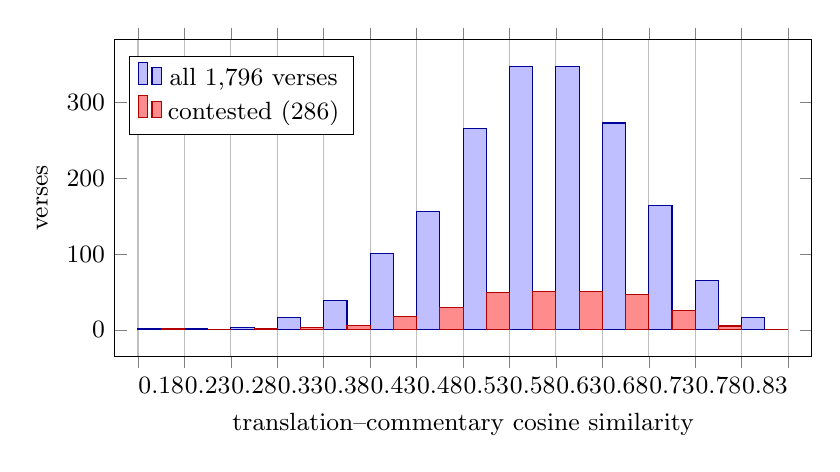
\begin{tikzpicture}
\begin{axis}[width=0.86\textwidth, height=5.6cm, ybar interval,
  xmin=0.15, xmax=0.9, xlabel={translation--commentary cosine similarity},
  ylabel={verses}, legend style={font=\small, at={(0.02,0.95)}, anchor=north west},
  tick label style={font=\small}, label style={font=\small}]
\addplot+[fill=blue!25, draw=blue!60!black] coordinates {
(0.175,1) (0.225,1) (0.275,3) (0.325,16) (0.375,39) (0.425,101) (0.475,156)
(0.525,266) (0.575,348) (0.625,347) (0.675,273) (0.725,164) (0.775,65)
(0.825,16) (0.875,0)};
\addplot+[fill=red!45, draw=red!70!black] coordinates {
(0.175,1) (0.225,0) (0.275,1) (0.325,3) (0.375,6) (0.425,18) (0.475,29)
(0.525,49) (0.575,50) (0.625,51) (0.675,47) (0.725,26) (0.775,5) (0.825,0)
(0.875,0)};
\legend{all 1{,}796 verses, contested (286)}
\end{axis}
\end{tikzpicture}
\caption{GPU semantic audit: distribution of translation--commentary embedding
similarity over the full corpus, with the contested subset overlaid. Contested
verses shift left (means $0.578$ vs.\ $0.593$); the lowest tail is the review
queue.}
\label{fig:audit}
\end{figure}

\section{Results}
\label{sec:results}

\begin{table}[t]
\centering
\caption{Verification results for the complete Brahmak\={a}\d{n}\d{d}a.}
\label{tab:results}
\begin{tabular}{lr}
\toprule
Verse units formalized \& verified & 144 / 144 \\
Entity declarations                & 772 \\
Contract axioms / denials          & 610 / 178 \\
Accepted-reading claims (all proved adequate) & 449 \\
Rejected readings, \texttt{contradicted} (denial asserted) & 153 \\
Rejected readings, \texttt{unlicensed} (no axiom entails)  & 197 \\
Lean theorems (all by \texttt{decide}, zero \texttt{sorry}) & 549 \\
Homonym registry (terms / senses)  & 41 / 91 \\
Python gates (pytest)              & 180 \\
Ledger events (append-only)        & 96 \\
\bottomrule
\end{tabular}
\end{table}

Table~\ref{tab:results} summarizes the verified state; CI reproduces it from a
clean checkout (corpus gates, \texttt{lake build}, zero-\texttt{sorry} sweep).
Beyond the counts, the qualitative yield is a machine-checked map of \emph{how
Book~I can be mistranslated}: each of the 350 refutations is a specific,
named failure --- pari\d{n}\={a}ma for vivarta (1.1), grammar demoted from
discipline to convention (1.11--1.14), spho\d{t}a temporalized (1.75--1.77),
inference granted autonomy the text denies it (1.30--1.42), the corrupt form
elevated to equal standing with the correct (1.147--1.155) --- together a
negative image of the doctrine, in theorem form.

The edition is deployed as a static site (per-verse pages with Devanagari,
IAST, translation, commentary, contested notes, and per-verse proof status)
with the repository, contracts, kernel and ledger public.

\section{Discussion}
\label{sec:discussion}

\paragraph{What mechanization buys.} Three things, in our experience of
building this. \emph{Regression}: interpretive commitments, once contracted,
are protected --- an edit to verse 1.46's treatment of the inner word that
contradicts 1.1's identity axioms breaks the build. \emph{Explicitness}: the
contract format forced decisions (is \emph{ved\-a} here the corpus or the
eternal seed-order?) that prose translation lets one defer; the homonym
registry is a by-product catalogue of exactly those decisions.
\emph{Adversarial coverage}: requiring every contract to carry provably
failing rival readings institutionalizes the question ``what would it mean to
get this verse wrong?'' --- a question translators ask irregularly and
reviewers cannot ask at scale.

\paragraph{Limitations.} The entailment relation is deliberately shallow
(closure of literal claims under identity symmetry), so adequacy is
membership-like rather than inferential; a richer relation (e.g.\ transitive
sambandha chains, or defeasible generics) would strengthen the theorems at the
cost of decidability discipline. Contracts formalize the \emph{formalizable
core} of a verse, not its full rhetorical content. The six-sort ontology is
coarse --- persons, for instance, are shoehorned (the child of 1.121/1.151 as
epistemic subject). And the whole edifice inherits the interpretive standpoint
of one commentary; contracts keyed to rival commentaries (V\d{r}\d{s}abha,
Pu\d{n}yar\={a}ja) would turn inter-commentarial disagreement itself into
diffable, checkable data --- to us the most interesting extension.

\paragraph{On agents.} The swarm wrote in hours what would take a solo
formalizer months, and its failures were institutionally useful: every class
of agent error that occurred is now a mechanical gate. We suggest this as a
general pattern for LLM-assisted scholarship: design so that the interesting
question is never ``did the model hallucinate?'' but ``did the artifact pass
the gate?''

\section{Conclusion}
\label{sec:conclusion}

We introduced commentary-driven translation validation and delivered, for the
first time to our knowledge, a machine-verified translation layer for a
classical Sanskrit philosophical text: the complete Brahmak\={a}\d{n}\d{d}a of
the \emph{V\={a}kyapad\={\i}ya}, with 144 adequacy theorems and 350 compiled
refutations over a checksummed 1,796-verse edition, produced by a gated
agentic loop whose every acceptance is replayable from an append-only ledger.
The method treats the prover not as a reader of Sanskrit but as a keeper of
commitments --- and Bhart\d{r}hari, for whom the sentence's meaning is an
undivided whole only manifested by its parts, would perhaps have appreciated a
verifier that refuses to let the parts of a translation contradict the whole
of its commentary. Books~II and~III (1,652 verses), richer entailment, and
multi-commentary contracts are the open vine.

\paragraph{Availability.} Code, corpus, contracts, kernel, proofs, ledger and
the living edition: \url{https://github.com/SharathSPhD/vakya-vallari};
edition mirrors at \url{https://vakya-vallari.vercel.app} and
\url{https://huggingface.co/spaces/qbz506/vakya-vallari}.

\bibliographystyle{plainnat}
\bibliography{refs}

\end{document}
